\documentclass[preview]{standalone}

\usepackage{amsmath}
\usepackage{amssymb}
\usepackage{stellar}
\usepackage{definitions}
\usepackage{bettelini}
\usepackage{tikz}

\begin{document}

\id{divergence-theorem}
\genpage

\section{Divergence Theorem}

\begin{snippetdefinition}{vector-field-divergence-definition}{Divergence}
    Let
    \(F=(F_1,\ldots,F_n)\colon U\subseteq\realnumbers^n
    \fromto\realnumbers^n\) be of class \(\mathcal C^1\). Its
    \emph{divergence} is
    \[
        \operatorname{div}F
        =\sum_{i=1}^n\frac{\partial F_i}{\partial x_i}.
    \]
\end{snippetdefinition}

\begin{snippettheorem}{classical-divergence-theorem}{Divergence theorem}
    Let \(\Omega\subseteq\realnumbers^n\) be a bounded admissible domain
    with piecewise \(\mathcal C^1\) boundary, oriented by the outward unit
    normal \(\nu_e\). If
    \(F\in\mathcal C^1(U,\realnumbers^n)\) on an open neighborhood \(U\)
    of \(\overline\Omega\), then
    \[
        \int_\Omega\operatorname{div}F\,dx_1\cdots dx_n
        =\int_{\partial\Omega}F\cdot\nu_e\,dS.
    \]
\end{snippettheorem}

\begin{snippet}{divergence-theorem-fundamental-calculus-interpretation}
    The divergence theorem is a multidimensional fundamental theorem of
    calculus. If \(n=1\), \(\Omega=(a,b)\), and
    \(F\colon\realnumbers\fromto\realnumbers\), it becomes
    \[
        \int_a^bF'(x)\,dx=F(b)-F(a).
    \]
    The outward normals at \(a\) and \(b\) are \(-1\) and \(+1\), so the
    right-hand side is precisely the outward flux across the boundary.
\end{snippet}

\section{Planar Building Blocks}

\begin{snippetproposition}{planar-divergence-rectangle-proposition}{Divergence formula on a rectangle}
    Let \(\Omega=[a,b]\times[c,d]\) and
    \(F=(F_1,F_2)\in\mathcal C^1\) on a neighborhood of \(\Omega\). Then
    \[
        \iint_\Omega\operatorname{div}F\,dx\,dy
        =\int_{\partial\Omega}F\cdot\nu_e\,d\sigma.
    \]
\end{snippetproposition}

\begin{snippetproof}{planar-divergence-rectangle-proposition-proof}{planar-divergence-rectangle-proposition}{Divergence formula on a rectangle}
    For the first component, the fundamental theorem of calculus gives
    \begin{align*}
        \iint_\Omega\frac{\partial F_1}{\partial x}\,dx\,dy
        &=\integral[c][d]
        [\integral[a][b][\partial_xF_1(x,y)][x]][y]\\
        &=\integral[c][d][F_1(b,y)-F_1(a,y)][y].
    \end{align*}
    The horizontal sides have zero \(x\)-component of the normal, while the
    vertical sides have normals \((1,0)\) and \((-1,0)\). Hence
    \[
        \iint_\Omega\partial_xF_1\,dx\,dy
        =\int_{\partial\Omega}F_1(\nu_e)_1\,d\sigma.
    \]
    Interchanging \(x\) and \(y\) yields the analogous identity for
    \(\partial_yF_2\). Adding them proves the formula.

    \begin{center}
        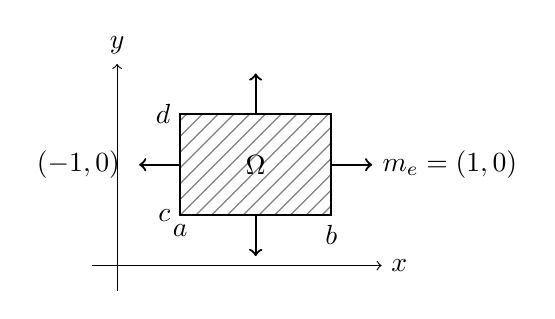
\begin{tikzpicture}[scale=0.8]
            \draw[->] (-0.4,0) -- (4.2,0) node[right] {\(x\)};
            \draw[->] (0,-0.4) -- (0,3.2) node[above] {\(y\)};

            \begin{scope}
                \clip (1,0.8) rectangle (3.4,2.4);
                \foreach \t in {-1.0,-0.75,...,3.4}{
                    \draw[gray] (\t,0.3) -- ++(2.6,2.6);
                }
            \end{scope}

            \draw[thick] (1,0.8) rectangle (3.4,2.4);

            \node[below] at (1,0.8) {\(a\)};
            \node[below] at (3.4,0.8) {\(b\)};
            \node[left] at (1,0.8) {\(c\)};
            \node[left] at (1,2.4) {\(d\)};
            \node at (2.2,1.6) {\(\Omega\)};

            \draw[->,thick]
                (3.4,1.6) -- (4.05,1.6)
                node[right] {\(m_e=(1,0)\)};

            \draw[->,thick]
                (1,1.6) -- (0.35,1.6);
            \node[left] at (0.20,1.6) {\((-1,0)\)};

            \draw[->,thick] (2.2,2.4) -- (2.2,3.05);
            \draw[->,thick] (2.2,0.8) -- (2.2,0.15);
        \end{tikzpicture}
    \end{center}
\end{snippetproof}

\begin{snippetproposition}{planar-divergence-axis-simple-proposition}{Component formula on an axis-simple domain}
    Let
    \[
        \Omega=
        \{(x,y):c\leq y\leq d,\ \alpha(y)\leq x\leq\beta(y)\},
    \]
    where \(\alpha\) and \(\beta\) are piecewise \(\mathcal C^1\). If
    \(F_1\in\mathcal C^1(\overline\Omega)\), then
    \[
        \iint_\Omega\partial_xF_1\,dx\,dy
        =\int_{\partial\Omega}F_1(\nu_e)_1\,d\sigma.
    \]
\end{snippetproposition}

\begin{snippetproof}{planar-divergence-axis-simple-proposition-proof}{planar-divergence-axis-simple-proposition}{Component formula on an axis-simple domain}
    Direct integration gives
    \[
        \iint_\Omega\partial_xF_1\,dx\,dy
        =\integral[c][d]
        [F_1(\beta(y),y)-F_1(\alpha(y),y)][y].
    \]
    Parametrize the two lateral curves by
    \[
        \gamma_\beta(y)=(\beta(y),y),
        \qquad
        \gamma_\alpha(y)=(\alpha(y),y).
    \]
    Their outward normals and arc elements are
    \[
        \nu_\beta=
        \frac{(1,-\beta')}{\sqrt{1+(\beta')^2}},
        \quad
        d\sigma_\beta=\sqrt{1+(\beta')^2}\,dy,
    \]
    and
    \[
        \nu_\alpha=
        \frac{(-1,\alpha')}{\sqrt{1+(\alpha')^2}},
        \quad
        d\sigma_\alpha=\sqrt{1+(\alpha')^2}\,dy.
    \]
    The length factors cancel, leaving the same difference of boundary
    values. The horizontal pieces contribute nothing to the first normal
    component.

    \begin{center}
        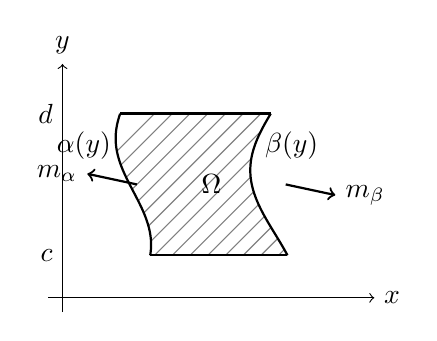
\begin{tikzpicture}[scale=0.9]
            \draw[->] (-0.2,0) -- (4.4,0) node[right] {\(x\)};
            \draw[->] (0,-0.2) -- (0,3.3) node[above] {\(y\)};

            \begin{scope}
                \clip
                    plot[domain=0.6:2.6,smooth,samples=100,variable=\t]
                        ({1+0.25*sin(120*\t)},{\t})
                    --
                    plot[domain=2.6:0.6,smooth,samples=100,variable=\t]
                        ({3+0.35*cos(100*\t)},{\t})
                    -- cycle;

                \foreach \s in {-1.2,-0.95,...,3.2}{
                    \draw[gray] (\s,0.1) -- ++(2.9,2.9);
                }
            \end{scope}

            \draw[thick,domain=0.6:2.6,smooth,samples=100,variable=\t]
                plot ({1+0.25*sin(120*\t)},{\t});

            \draw[thick,domain=0.6:2.6,smooth,samples=100,variable=\t]
                plot ({3+0.35*cos(100*\t)},{\t});

            \draw[thick]
                ({1+0.25*sin(120*0.6)},0.6) --
                ({3+0.35*cos(100*0.6)},0.6);

            \draw[thick]
                ({1+0.25*sin(120*2.6)},2.6) --
                ({3+0.35*cos(100*2.6)},2.6);

            \node[left] at (0,0.6) {\(c\)};
            \node[left] at (0,2.6) {\(d\)};

            \node at (2.1,1.6) {\(\Omega\)};

            \node[left] at (0.82,2.15) {\(\alpha(y)\)};
            \node[right] at (2.72,2.15) {\(\beta(y)\)};

            \draw[->,thick]
                (3.15,1.6) -- (3.85,1.45)
                node[right] {\(m_\beta\)};

            \draw[->,thick]
                (1.05,1.6) -- (0.35,1.75)
                node[left] {\(m_\alpha\)};
        \end{tikzpicture}
    \end{center}
\end{snippetproof}

\begin{snippetproposition}{divergence-finite-domain-decomposition-proposition}{Finite decomposition of domains}
    Suppose an admissible domain \(\Omega\) is the union of finitely many
    admissible domains with pairwise disjoint interiors, and the divergence
    theorem holds on each piece. Then it holds on \(\Omega\).
\end{snippetproposition}

\begin{snippetproof}{divergence-finite-domain-decomposition-proposition-proof}{divergence-finite-domain-decomposition-proposition}{Finite decomposition of domains}
    For two pieces \(\Omega=\Omega_1\cup\Omega_2\), add the two divergence
    identities. Volume integrals add because the interiors are disjoint.
    Every common boundary portion is traversed with opposite outward normals
    for the two pieces, so its flux contributions cancel. Only the exterior
    boundary of \(\Omega\) remains. The finite case follows by induction.

    \begin{center}
        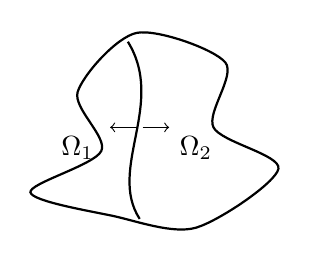
\begin{tikzpicture}[scale=0.75]
            \draw[thick] plot[smooth cycle] coordinates {(0,0) (1.2,0.7) (0.8,1.7) (1.8,2.7) (3.3,2.2) (3.1,1.1) (4.2,0.4) (2.8,-0.6) (1.4,-0.4)};
            \draw[thick] (1.85,-0.45) .. controls (1.3,0.4) and (2.3,1.5) .. (1.65,2.55);
            \node at (0.8,0.75) {\(\Omega_1\)};
            \node at (2.8,0.75) {\(\Omega_2\)};
            \draw[->] (1.8,1.1) -- (1.35,1.1);
            \draw[->] (1.9,1.1) -- (2.35,1.1);
        \end{tikzpicture}
    \end{center}
\end{snippetproof}

\end{document}
